\documentclass[10pt]{article}
\usepackage[margin=1cm]{geometry}
\usepackage{setspace}
\setstretch{0.9}

\usepackage{enumitem}\setlist[itemize]{topsep=0pt}
\usepackage{amssymb}
\usepackage{amsmath}
\usepackage{fancybox}
\usepackage{graphicx}
\usepackage{fancyvrb}
\usepackage[most]{tcolorbox}


\usepackage{cse571}
\raggedright
\pagestyle{empty}
\pagenumbering{gobble}
\begin{document} \noindent

\section*{cse571 midterm review}

bayseian network conditional indepedence: use markov blanket for belief propagation
\hspace{2em}
\begin{minipage}[b]{0.6\textwidth}
    for nodes in $\mathbf{A} \subset \mathbf{N}$ where
    \begin{itemize}[leftmargin=1em, itemsep=-0.3em]
        \item[] $\mathbf{N}$:= universe of all nodes in network
        \item[] $\mathbf{B}$:= $blanket(\mathbf{A})$, markov blanket (neighbours) of nodes in $\mathbf{A}$
        \item[] $\mathbf{C}$:= $\mathbf{N}\setminus(\mathbf{A} \cup \mathbf{B})$, nodes not in $\mathbf{A}$ or $\mathbf{B}$
    \end{itemize}
    conditional indepedence: $(\mathbf{A}\condind \mathbf{C})\ |\ \mathbf{B}$\\
\end{minipage}
\begin{minipage}[b]{0.2\textwidth} \footnotesize
    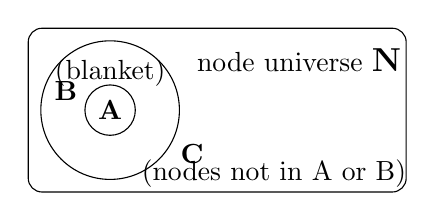
\begin{tikzpicture}[scale=0.8]
        \def\setcircle{(1.4,1.4) coordinate (a) circle (0.4)}
        \def\blanket{(1.4,1.4) coordinate (b) circle (1.1)}
        \def\universe{(0.1,0.1) coordinate (u) rectangle (6.1,2.7)}
        % \begin{scope}
        %     \fill[yellow!40] \universe;
        %     \clip \blanket;
        %     \fill[magenta!40] \blanket;
        %     \clip \setcircle;
        %     \fill[cyan!50] \setcircle;
        % \end{scope}
        \draw \setcircle node at (1.4,1.4) {$\mathbf{A}$};
        \draw \blanket node at (0.7,1.7) {$\mathbf{B}$};
        \node at (1.4,2) {(blanket)};
        \draw[rounded corners=5pt] \universe node at (4.4,2.2) {node universe \large $\mathbf{N}$};
        \node at (2.7,0.7) {$\mathbf{C}$};
        \node at (4,0.4) {(nodes not in A or B)};
    \end{tikzpicture}
\end{minipage}

\begin{table}[h]
    \small
    \begin{tabular}{|c|c|c|c|c|} \hline
        rectified linear unit                                                                                           & sigmoid & hyperbolic tangent & exponential linear unit & softmax
        \\ \hline
        $relu(x) = max(0, x)$                                                                                           &
        $\sigma(x) = \displaystyle\frac{1}{1 + e^{-x}}$                                                                 &
        $tanh(x) = \displaystyle\frac{e^{x} - e^{-x}}{e^{x} + e^{-x}}$                                                  &
        $elu(x) = \begin{cases} x & x > 0 \\ \alpha(e^{x} - 1) & x \leq 0 \end{cases}$                                  &
        $softmax_i(x) = \displaystyle\frac{e^{x_i}}{\sum e^{x_k}}$
        \\
        $\displaystyle \frac{\partial}{\partial x} = \begin{cases} 1 & x > 0 \\ 0 & x \leq 0 \end{cases}$               &
        $\displaystyle \frac{\partial}{\partial x} = \sigma(x)(1: \sigma(x))$                                           &
        $\displaystyle \frac{\partial}{\partial x} = 1 - tanh^2(x)$                                                     &
        $\displaystyle \frac{\partial}{\partial x} = \begin{cases} 1 & x > 0 \\ elu(x) + \alpha & x \leq 0 \end{cases}$ &
        \\\hline
        %                                                                                                                 &         &                    &                         &
        % \rule{0pt}{5em}                                                                                                                                                                    \\ \hline
    \end{tabular}
\end{table}

\section*{week 1: intro to machine learning}

\subsection*{from week1(ML) practice questions}
\begin{itemize}[label=\(\star\), leftmargin=1em, itemsep=-0.3em]
    \item supervised learning: model learns mapping of input to output
    \item high generalization: make accurate predictions/classifications on new/unseen data
    \item loss/cost/error function: minimize distance to target labels
    \item functional view maps inputs to outputs (vs) probabilistic view calculates conditional probability distributions based on inputs
    \item reinforcement learning: sequential decisions, explore actions and observe consequences, optimize reward/punishment (manually specified), autonomy, trial\&error, learn policy for realtime decisions
    \item RL policy: takes state as input and outputs action, can be deterministic or stochastic, maximizes expected cumulative reward over time
    \item binning: approximate joint distribution over variables, capture discrete patterns/categories, non-linear relationships, relationships with by distinct ranges/intervals rather than continuous function (regression)
    \item dimentionality reduction: manifold learning, reduce number of features (and noise, computational cost)
    \item stochastic gradient descent: update model params based on average gradient computed from mini-batch (randomly selected subset of training data), memory-efficient, adds noise to escape local minima, makes an update step for each sample
    \item qubits: quantum bits, can hold an exponential number of states using superposition (of 0 and 1) and entanglement (for parallel computation)
    \item QML rotation embedding: relatively simple to implement, uses only linear number of qubits
    \item if normalization is not performed on input data features that have higher values will influence network more, and very small values will have no effect at all - quality of learning decreases
    \item in QML, data embedding requires storing classical data in quantum states
    \item in QML, amplitude encoding  has higher qubit requirement than rotation encoding
    \item ansatz (in qml) typically refers to designing structure and layers of neural network
\end{itemize}

\pagebreak
\section*{week 2: intro to neural networks}

\subsection*{from week2(NN) practice questions}
\begin{itemize}[label=\(\star\), leftmargin=1em, itemsep=-0.3em]
    \item training time: depends on convergence rate
    \item early-stopping: stop training when validation loss starts increase, may require more iterations of training to find optimal model
    \item activation function: must be non-linear (eg sigmoid, tanh, ReLU, softmax), should be computationally efficient
    \item update step of gradient descent: $weight_{new} = weight_{old}: learning\_rate * gradient$, learning rate determines size of step taken in direction of gradient
    \item softmax outputs a probability distribution over multiple classes (vs) sigmoid outputs a single probability for binary classifications
    \item softmax: outputs a probability distribution over multiple classes, sum of all probabilities is 1, used for multi-class classification
    \item forward pass: input is multiplied by weights and added to bias, then passed through activation function
    \item back-propagation objective: minimize loss function to make predictions closer to target values
    \item back-propagation algorithm (for fully connected feed-forward NN): after forward passes of input produces output, calculate loss wrt output and target weight (based on loss function) and use chain rule to calculate gradient of loss function wrt weights/biases of each layer, then update weights using gradients and learning rate
    \item normalize dataset before training when features have different scales
    \item cross-entropy loss: difference between predicted probabilities and true labels (target probability distribution), used for classification problems
    \item mean-squared error: difference between predicted values and true values, used for regression problems
\end{itemize}

\subsection*{from week2(NN) lectures}
\begin{itemize}[label=\(\star\), leftmargin=1em, itemsep=-0.3em]
    \item output from activation function is continuous (vs) output from step function is discrete
    \item standard forward pass (taking input through NN to produce output) is deterministic (vs) stochastic forward pass adds noise
    \item every neuron connection must have weight parameter, and has bias parameter
    \item NN is bested function of layers of neurons, each layer is a function of previous layer
    \item back propagation: partial derivatives via chain rule, provide gradient information that is needed for gradient descent, determine parameter updates to minimize training error, requires dataset of inputs and target outputs to generate network output and calculate discrepancy via loss function, calculate gradient of this loss function with respect to model parameters
    \item paritial derivative of loss function wrt param changes based on depth of parameters
    \item output of each neuron's activation function in final layer is output of NN
    \item must forward propgate before every backward propagation when training model
    \item neural turing machines (NTM): combine learning capabilities of neural networks with ability to read and write to external memory like a traditional turing machine
    \item pytorch: loss.backward(), torch.nn.Module, torch.nn.Linear connects any fully connected layers, optimizer determines how to update our parameters based on calculated gradient (eg sgd, adam)
    \item if derivative cannot be computed algebraically, numerically approximate limit found in definition of derivatives
    \item k-fold cross-validation: validate or reject suspicion of overfitting
        \begin{enumerate}[leftmargin=1em, itemsep=-0.3em]
            \item shuffle dataset randomly,
            \item split dataset into k groups/folds
            \item for each group: take group as a hold out or test data set
            \item for each group: take remaining groups as a training data set
            \item for each group: fit a model on training set and evaluate it on test set
            \item for each group: retain evaluation score and discard model
            \item summarize skill of model using sample of model evaluation scores
        \end{enumerate}
    \item ADAM (Adaptive Moment Estimation): considers curvature
\end{itemize}

\pagebreak
\section*{week 3: recurrent neural networks}

\subsection*{from week3(RNN) practice questions}
\begin{itemize}[label=\(\star\), leftmargin=1em, itemsep=-0.3em]
    \item name classification: sequence labeling, each element in input sequence is assigned a label, each label is independent of other labels
    \item sequence generation: generate a sequence of outputs (eg sentence/paragraph, series of actions)
    \item sequence-to-sequence: input and output are both sequences,transforms an input sequence into an output sequence, (eg machine translation)
    \item gradient clipping: limit max value of gradient to prevent exploding gradients, not solution to vanishing gradients, can limit step size during training and hinder learning, this is because it artificially restricts updates to model parameters, can distort gradients/learning process resulting in suboptimal convergence or longer training time
    \item monte carlo dropout: regularization, same model runs multiple times with different dropout masks, not multiple different models, adds noise from randomly dropping units (setting their outputs to zero), not by adding Gaussian noise to activations (stochastic noise injection), using dropout at test time to sample predictions
        \begin{itemize}[label=\(\star\),leftmargin=1em, itemsep=-0.3em]
            \item mcd makes inference non-determinstic (vs) NN inference is deterministic in generalization
            \item output of NN using mcd a set of inferences: can treat this set as a normal distribution and use mean of this distribution as prediction and variance as a metric of its certainty in that prediction
        \end{itemize}
    \item number of dropout layer config: $n$ neurons, $p$ dropout probability, $np$ number of neurons expected to dropout, number of configs = $(n\,{\operatorfont{C}}\,np)$
    \item number of trainable parameters
    \item RNN forward pass: $h_t = \sigma(Ux_t + Wh_{t-1} + b)$, $y_t = \phi(Vh_t) + b$
    \item LSTM new information
          \begin{itemize}[label=\(\star\),leftmargin=1em, itemsep=-0.3em]
              \item input gate: $i_t = \sigma(U_i x_t + W_i h_{t-1} + b_i)$, sigmoid output $\in (0,1)$ to decides how much of each value to let through
              \item forget gate: $f_t = \sigma(U_f x_t + W_f h_{t-1} + b_f)$, decides which parts of cell state $C_{t-1}$ to forget
              \item output gate: $o_t = \sigma(U_o x_t + W_o h_{t-1} + b_o)$, decides what parts of cell state $C_t$ to output to hidden state $h_t$
              \item new candidate values: $\tilde{C}_t = tanh(U_c x_t + W_c h_{t-1} + b_C)$, new candidate values that could be added to state, $tanh$ output $\in [-1,1]$ to provide candidate values
              \item cell state: $C_t = f_t \odot C_{t-1} + i_t \odot \tilde{C}_t$, updates cell state where old state $C_{t-1}$ is forgotten according to forget gate $f_t$, and new candidate values are added scaled by input gate $i_t$.
              \item hidden state: $h_t = o_t \odot tanh(C_t)$, cell state $C_t$ is passed through $tanh$ to push values $\in [-1,1]$ range, then multiplied by output of output gate $o_t$ to decide which parts to keep
              \item gates use sigmoid, hidden state uses $tanh$
              \item drawback: requires training for many more parameters
              \item advantage: handling data with dependencies on very distant time steps, solves vanishing
          \end{itemize}
    \item feedforward NN not best for period series: does not utilize temporal information, does not have memory, does not have feedback loops
    \item one-hot encoding: convert each categorical value, assign a binary value of 1/0, each integer value is represented as a binary vector,size of input vector at each time step is equal to number of unique values in categorical variable
\end{itemize}

\subsection*{from week3(RNN) lectures}
\begin{itemize}[label=\(\star\), leftmargin=1em, itemsep=-0.3em]
    \item passing info to next step: hidden state is multiplied by its own weight matrix and added to same layer at next sequence step - having an independent weight matrix allows greater control of what gets passed on through time
    \item recurrent backpropagation: calculates update gradients for RNN, calculating partial derivatives with respect to terms in prior step
    \item leverage temporal features of dataset
    \item unfolding: visualizing or representing network over time or through its sequential steps
    \item backpropagation through time: backpropagation through an unfolded RNN
    \item when using chain rule to connect loss function to parameters in a prior timestep, connection is made via every hidden state between loss and parameter at timestep
    \item vanishing gradients: gradients get smaller and smaller at an increasing rate for every step backward (exponential decay), can be caused by activation functions with small gradients (eg sigmoid, tanh which squash their input into a narrow range and have derivatives close to zero for inputs far from zero)
        \begin{itemize}[label=\(\star\), leftmargin=1em, itemsep=-0.3em]
            \item magnitude of weights connecting hidden state are less than 1
            \item can be caused by deep networks with many layers, can be caused by long-term dependencies in RNNs
            \item initialization solution: ensure eigenvalues of recurrent weight matrix are equal to one, soft constraints imposed on matrices improve trainability (eg identity and orthogonal initialization of weight matrice)
            \item timesteps further removed (in time) from network's output have little to no influence on VANISHING gradients:
                \begin{itemize}[label=\(\star\), leftmargin=1em, itemsep=-0.3em]
                    \item nature of backpropagation through time in recurrent neural network: gradient of loss function with respect to weights tends to get smaller with each timestep, especially when activation functions squash their inputs into a narrow range, leading to small derivatives
                    \item results in weights associated with earlier timesteps (further removed in time) receive very small updates, and have little to no influence on learning of network
                \end{itemize}
        \end{itemize}
    \item exploding gradients: gradients get larger and larger at an increasing rate for every step backward, can be caused by activation functions with large gradients (eg sigmoid, tanh), can be caused by deep networks with many layers, can be caused by long-term dependencies in RNNs, magnitude of weights connecting hidden state are greater than 1
        \begin{itemize}[label=\(\star\), leftmargin=1em, itemsep=-0.3em]
            \item gradient clipping solution: limit max value of gradient to prevent exploding gradients, not solution to vanishing gradients, can limit step size during training and hinder learning, this is because it artificially restricts updates to model parameters, can distort gradients/learning process resulting in suboptimal convergence or longer training time, evaluate norm and rescale to allowed
            threshold
            \item weights associated with earlier timesteps (further removed in time) receive very large updates, and have large influence on learning of network
        \end{itemize}
    \item tanh: outputs a value between -1 and 1, used for classification problems, gradient vanishes more quickly further x deviates from 0
    \item relu: outputs a value between 0 and 1, used for classification problems,  has desirable gradient behavior for values of x > 0, for x < 0 temporal gradient does not exist, ensures that feature map values are always positive
    \item current hidden state is a function of all prior hidden states and all prior and current inputs
    \item LSMT: long short-term memory, uses gates to control flow of information, can learn long-term dependencies, can learn to forget information, append predictions to known input sequence to feed new input elements over arbitrary distances
    \begin{itemize}[label=\(\star\), leftmargin=1em, itemsep=-0.3em]

        \item LSTM forget gates: adds new gate to LSTM architecture that focuses on “forgetting” longterm dependencies that are no longer relevant
        \item peephole LSTM: uses previous cell state for gate computations instead of hidden state; accesses constant error carousel
    \end{itemize}
    \item GRU: gated recurrent unit, combines input and forget gates into single update gate and combines cell and hidden memory states
    \item GNN: graph neural network
    \item IndRNN: forces recurrent weight matrix to be a vector that is multiplied element-wise by previous hidden state
    \item UGRNN: modern architectures made to enhance trainability of deeply-stacked (RNN+) and shallow (UGRNN) models
    \item softmax: outputs a probability distribution over multiple classes, sum of all probabilities is 1, used for multi-class classification, output is highest probability class
    \item dropout: regularization, adds noise from randomly dropping units (setting their outputs to zero), not by adding Gaussian noise to activations (stochastic noise injection), using dropout at test time to sample predictions
    \begin{itemize}[label=\(\star\), leftmargin=1em, itemsep=-0.3em]
        \item network trained with dropout produces output that approximates mean of multiple networks
        \item network trained with dropout approximates mean of multiple NN outputs
        \item matrix multiplication operation to implement dropout at test time: multiply each weight by probability of keeping that weight
        \item at inference time: scale activations on dropout layers by dropout probability
        \item dropout all connections from a neuron to next layer by multiplying activation by 0
        LSTM forget gates: adds new gate to LSTM architecture that focuses on “forgetting” longterm dependencies that are no longer relevant
        \item peephole LSTM: uses previous cell state for gate computations instead of hidden state; accesses constant error carousel
    \end{itemize}
\end{itemize}

\pagebreak
\section*{week 4: convolutional neural networks}

\subsection*{from week4(CNN) practice questions}
\begin{itemize}[label=\(\star\), leftmargin=1em, itemsep=-0.3em]
    \item edge detection: image processing, identify boundaries of objects within images, detecting discontinuities in brightness (eg Sobel, Prewitt, Canny algorithms)
    \item points of interest (key/feature points): image processing, identify corners/colors/distinctive visual features, image processing (e.g, SIFT Scale-Invariant Feature Transform, SURF Speeded Up Robust Features algorithms)
    \item stop-word removal: NLP, remove common words (eg the, a, for), reduce dimensionality of text data, reduce noise, reduce computational cost
    \item denoising: remove noise from data (eg random color variation in images, background noise in audio processing)
    \item sharpening filter kernel: high value at center of kernel to enhance center pixel on each stride
    \item blurring filter kernel: ability to reduce noise, gaussian distribution filter (more weight to pixels near center of kernel and less weight to pixels further away), box filter
    \item box filter: uniform, box-like structure, equal weight to all pixels in kernel, results in a blurring efficient
    \item flattening: connect outputs from convolution section into classifier section (fully connected layers of CNN), convert 2D feature maps outputted by convolutional layers into a 1D vector (fully connected layers (which typically make up classifier section of a CNN) expect input in form of a 1D vector), reshapes output of preceding layer (does not combine layers, nor apply non-linear activation functions to feature maps),  must be performed on feature maps in order to pass them to fully connected layers
    \item ML form and function iterate and inform each other
    \item kernel transform an image by linearly combining pixel regions
\end{itemize}

\subsection*{from week4(CNN) lectures \& quizzes}
\begin{itemize}[label=\(\star\), leftmargin=1em, itemsep=-0.3em]
    \item GAN: generative adversarial network, generator and discriminator (adversarial network), generator learns to generate realistic data, discriminator learns to distinguish between real and fake data, generator learns to fool discriminator, discriminator learns to not be fooled by generator
    \item CNN: convolutional neural network, uses convolutional layers to learn features, uses pooling layers to reduce spatial dimensionality, uses fully connected layers to learn non-linear combinations of features
    \begin{itemize}[label=\(\star\), leftmargin=1em, itemsep=-0.3em]
        \item learning kernels that can be universally applied to entire image instead of weights for every individual pixel and channel
        \item through each convolutional layer, channels increase and pixel width and height decrease in general

    \end{itemize}
    \item pooling: reduces spatial dimensionality
    \item fully connected layer: learns non-linear combinations of features, learns non-linear decision boundaries, learns non-linear relationships between features, connect feature map values to a classification
    \item regularization: reduces overfitting, reduces model complexity, reduces number of parameters, reduces model variance, increases model bias
    \item convolutional layer: runs kernels over regions of pixels in a digital image, learns useful kernel for each feature map
    \item key purpose of pooling layer: is reducing spatial dimension as number of channels generally increases
    \item different feature maps generated for same image within a CNN by convolving different kernels - feature map will be created for each kernel applied
    \item stride: number of pixels shifted between each convolution, horizontal and vertical pixel step size of each convolution
    \item repeatable convolutional component: convolutional layer, pooling layer, activation function
    \item log probability:
    \begin{itemize}[label=\(\star\), leftmargin=1em, itemsep=-0.3em]
        \item take in an input image and output a log probability for each class
        \item efficient computation, addition replaces multiplication operation
        \item yields only negative values, values closer to 0 are more likely
    \end{itemize}
\end{itemize}




\end{document}
